\documentclass[a4paper]{article}
\usepackage[utf8]{inputenc}
\usepackage[spanish]{babel}
\usepackage{amsmath}
\usepackage[margin=1.5cm]{geometry}
\usepackage{graphicx}
\usepackage{caption}
\usepackage{subcaption}
\usepackage{float}

\numberwithin{equation}{section}

\title{Notas de Física 2}
\author{S. Schiavinato}


\begin{document}
\maketitle
\tableofcontents
\section{Oscilador armónico}
    Todo movimiento podemos clasificarlo como acotado o no acotado. Los movimientos acotados son los que nos van a interesar analizar en estas primeras secciones. Además de los movimientos acotados también vamos a describir los movimientos oscilatorios, es decir los cuales que varían de forma estable (o no, esto ya depende de la definición precisa) respecto a estado de equilibrio (donde las razones dinámicas, las fuerzas, del movimiento no existen). 
    El ejemplo más simple de oscilador es un resorte con una masa (en el vacío y sin gravedad, para simplificarlo más aún). Tomamos como otra consideración que el movimiento va a ser unidimensional. Aplicando las ecuaciones de Newton encontramos que el movimiento está dado por
    \begin{equation*}
        \ddot{x}(t) = - \frac{k}{m} x(t)
    \end{equation*}
    y tiene por solución la siguiente ecuación
    \begin{equation*}
        x(t) = A \sen(\omega_0 t + \phi_0)
    \end{equation*}
    siendo $A$ y $\phi_0$ condiciones iniciales (derivables de $x(t = 0)$ y $\dot{x}(t = 0)$), y $\omega_0 = \sqrt{\dfrac{k}{m}}$ la frecuencia angular de oscilación. 
    Podemos encontrar muchos fenómenos físicos que sean modelables con la ecuación del resorte, y todos ellos los podemos describir con la ecuación \ref{eq:oscilador}, la denominada ecuación del oscilador armónico (con una frecuencia definida)
    \begin{equation}
        \ddot{\psi} = -\omega_0^2 \psi
        \label{eq:oscilador}
    \end{equation}
    donde la constante $\omega_0$ representa la frecuencia de oscilación de la coordenada $\psi$, que no necesariamente va a ser unidad de fuerza por unidad de masa sobre unidad de distancia como el caso del resorte. Con la ecuación anterior tenemos como solución general
    \begin{equation}
        \psi(t) = A e^{i \omega_0 t} + B e^{-i \omega_0 t} + cc = C e^{i (\omega_0 t + \phi_0)} = A \sen_(\omega_0 t + \phi_0)
        \label{eq:oscilador_solucion}
    \end{equation}
    Todas las expresiones son soluciones posibles, todas dan soluciones reales (ya que cc significa complejo conjugado) y básicamente son senos y cosenos sumados, o un seno/coseno con una fase inicial.
    Ahora veamos la energía del oscilador en general, considerando que $\omega_0^2 = \dfrac{k}{m}$, siendo $k$ y $m$ las magnitudes que correspondan dependiendo del caso.
    \begin{equation}
        E = \frac{1}{2} m \dot{\psi}(t)^2 + \frac{1}{2} k \psi(t)^2
        \label{eq:oscilador_energia}
    \end{equation}
    de donde observamos que la energía cinética es cuadrática con las velocidades generalizadas y la energía potencial cuadrática con la posición. Con la solución \ref{eq:oscilador_solucion} observamos que la energía se conserva tiempo a tiempo y que tiene la siguiente expresión
    \begin{equation}
        E(t) = \frac{1}{2} k A^2
        \label{eq:oscilador_energia_tiempo}
    \end{equation}
    es decir, que una de las condiciones iniciales depende de la energía inicial.
    \subsection{Oscilador con disipación viscosa}
    Podemos agregarle al oscilador armónico una fuerza dependiente de la velocidad, que hace que la energía del sistema se disipe y se amortigue el movimiento. Es decir, la forma funcional general del oscilador armónico amortiguado es
    \begin{equation}
        \ddot{\psi} = - \omega_0^2 \psi - \gamma \dot{\psi}
        \label{eq:oscilador_amortiguado}
    \end{equation}
    con tres soluciones posibles, que se derivan de la ecuación algebraica característica $\lambda^2 + \gamma \lambda + \omega_0^2 = 0$, la solución subamortiguada
    \begin{equation}
        \psi(t) = A e^{-\alpha t} e^{i (\omega t + \phi_0)},
        \label{eq:oscilador_amortiguado_sub}
    \end{equation}
    mientras que la solución críticamente amortiguada es
    \begin{equation}
        \psi(t) = (A + B t) e^{\alpha t}
        \label{eq:oscilador_amortiguado_critico}
    \end{equation}
    Finalmente la solución sobreamortiguada es
    \begin{equation}
        \psi(t) = A e^{(-\alpha + \omega) t} + B e^{(-\alpha - \omega) t}
        \label{eq:oscilador_amortiguado_critico}
    \end{equation}
    con $\alpha = \dfrac{\gamma}{2}$ y $\omega = \dfrac{\sqrt{\gamma^2 - 4 \omega^2}}{2}$ (en el caso subamortiguado este valor es complejo pero la unidad imaginaria la sacamos de la ecuación). Esas formas funcionales las podemos ver en el gráfico de la figura \ref{fig:oscilador_amortiguado}
	\begin{figure}[H]
		\centering
		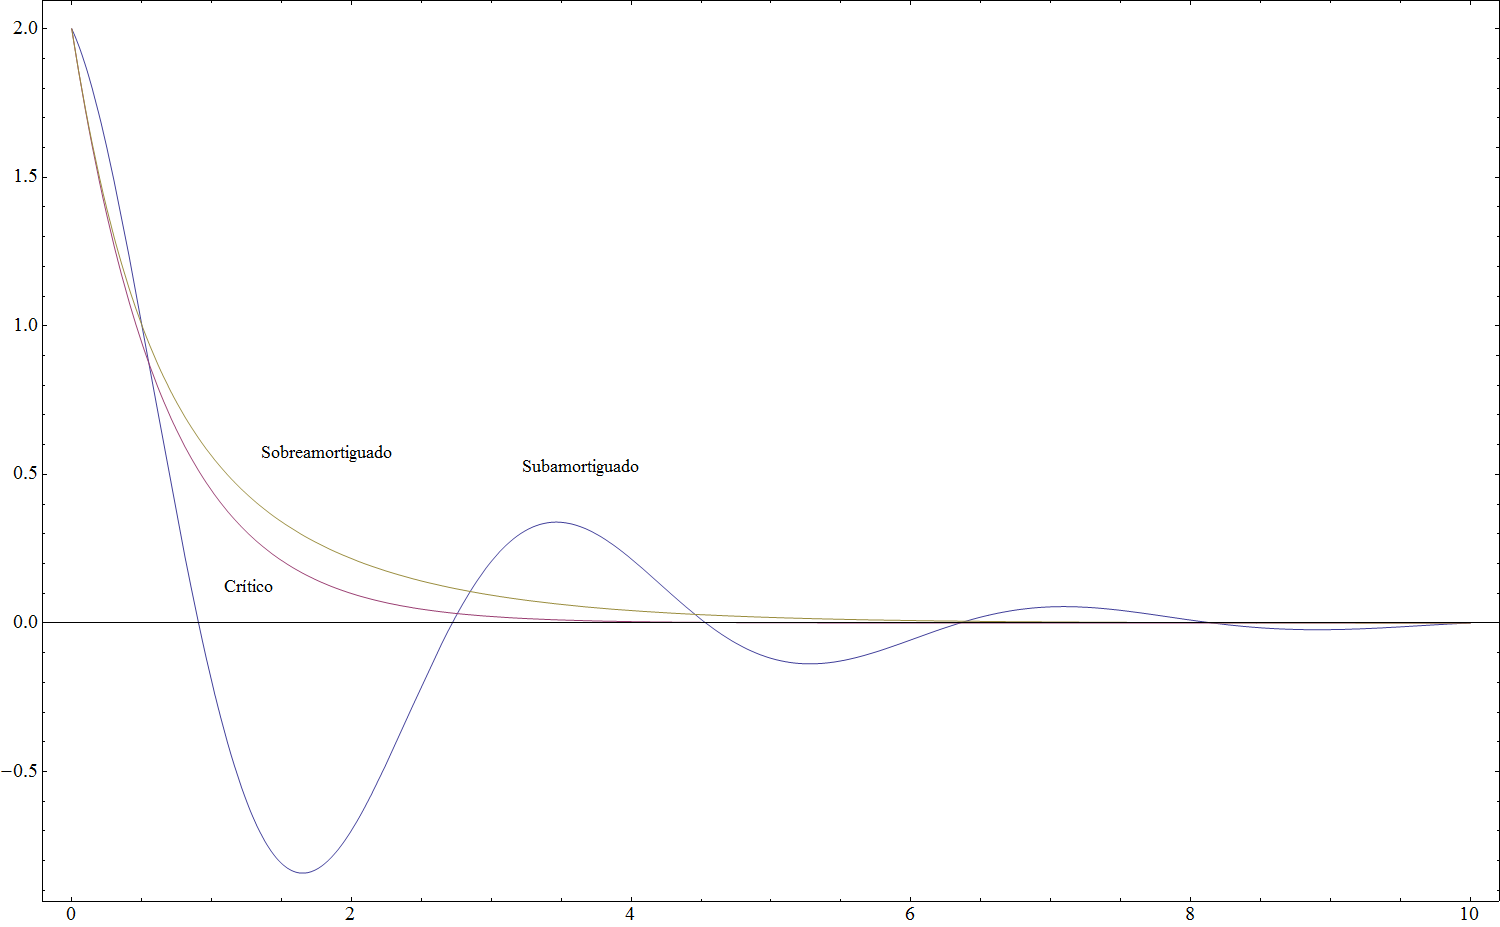
\includegraphics[scale=0.25]{amortiguado}
		\caption{Soluciones posibles para un oscilador amortiguado}
		\label{fig:oscilador_amortiguado}
	\end{figure}
    De esta forma la energía de la expresión \ref{eq:oscilador_energia} queda dependiente del tiempo, y vamos a expresarla solamente para el caso subamortiguado 
    \begin{equation}
        E(t) = E(t = 0) e^{-\alpha t}
        \label{eq:oscilador_amortiguado_energia}
    \end{equation}
    y definimos una magnitud denominada factor de mérito, que representa la cantidad de energía perdida por ciclo de la frecuencia $\omega$, es decir
    \begin{equation}
        Q = \frac{\omega_0}{\alpha}
    \end{equation}
	y con esa magnitud definimos que la energía perdida en un periodo $\tau = \dfrac{2\pi}{\omega}$ es
	\begin{equation}
		\Delta E = - \frac{2\pi}{Q} E(t=0)
	\end{equation}
    \subsection{Oscilador forzado}
	Ahora observemos el oscilador forzado (con rozamiento viscoso) por una fuente externa dependiente del tiempo, es decir
    \begin{equation}
        \ddot{\psi} = - \omega_0^2 \psi - \gamma \dot{\psi} + a(t)
        \label{eq:oscilador_forzado}
    \end{equation}
	Este oscilador lo resolvemos primero solucionando la parte homogénea (sin la fuente dependiente del tiempo) y luego la particular, para la cual solo algunas formas son fácilmente solucionables. Vamos a ver como solucionar con $a(t) = A \sen(\omega t)$. Intuitivamente sabemos que si la fuente externa pone la frecuencia de oscilación del sistema finalmente, pero que el sistema va a responder mejor si es parecida su frecuencia natural $\omega_0$. Proponiendo como solución particular $\psi = C e^{i \omega t}$ obtenemos la siguiente ecuación algebraica $(\omega_0^2 - \omega^2 + i \omega \gamma) C = A$, por lo que la amplitud es
	\begin{equation}
		C = \frac{A (\omega_0^2 - \omega^2 - i \omega \gamma)}{(\omega_0^2 - \omega^2)^2 + (\omega \gamma)^2} = \frac{A (\omega_0^2 - \omega^2)}{(\omega_0^2 - \omega^2)^2 + (\omega \gamma)^2} - i \frac{A \omega \gamma}{(\omega_0^2 - \omega^2)^2 + (\omega \gamma)^2}
		\label{eq:oscilador_forzado_particular_amplitud}
	\end{equation}
	y esto tiene como solución
	\begin{equation}
		\psi_p(t) = \Re(C) \cos(\omega t) + \Im(C) \sen(\omega t) = C' \cos(\omega t + \phi)
		\label{eq:oscilador_forzado_particular_solucion}
	\end{equation}
	que no tiene constante de integración ($\Re$ es la parte real y $\Im$ es la parte imaginaria) ya que dichas aparecen solamente en la solución homogénea. Además la solución homogénea decae, como se ve en la figura \ref{fig:oscilador_amortiguado}, por lo que luego de un tiempo (denominado transitorio) pasa a un estado estable o estacionario donde predomina la solución particular. La fase $\phi$ indica como está desfasado el movimiento de la solución particular de la solución homogénea.

	Veamos la potencia asociada al oscilador forzado, en el régimen estacionario donde $\psi \approx \psi_p$, la cual es igual a 
	\begin{equation}
		P(t) = a(t) \dot{\psi}(t) = A \sen(\omega t) \omega (- \Re(C) \sin(\omega t) + \Im(C) \cos(\omega t))
		\label{eq:oscilador_forzado_potencia_t}
	\end{equation}
	y si hacemos el promedio temporal en un periodo $\tau = \dfrac{2\pi}{\omega}$ obtenemos
	\begin{equation}
		<P(t)> = \frac{1}{2} A \omega \Re{C} = P_0  \frac{\gamma^2 \omega^2}{(\omega_0^2 - \omega)^2 + \gamma^2 \omega^2}
		\label{eq:oscilador_forzado_potencia_resonancia}
	\end{equation}
	donde vemos que si la frecuencia $\omega = \omega_0$ la potencia es máxima, efecto que denominamos resonancia. En la figura \ref{fig:resonancia} observamos el valor de la potencia en función de la frecuencia.
	\begin{figure}[H]
		\centering
		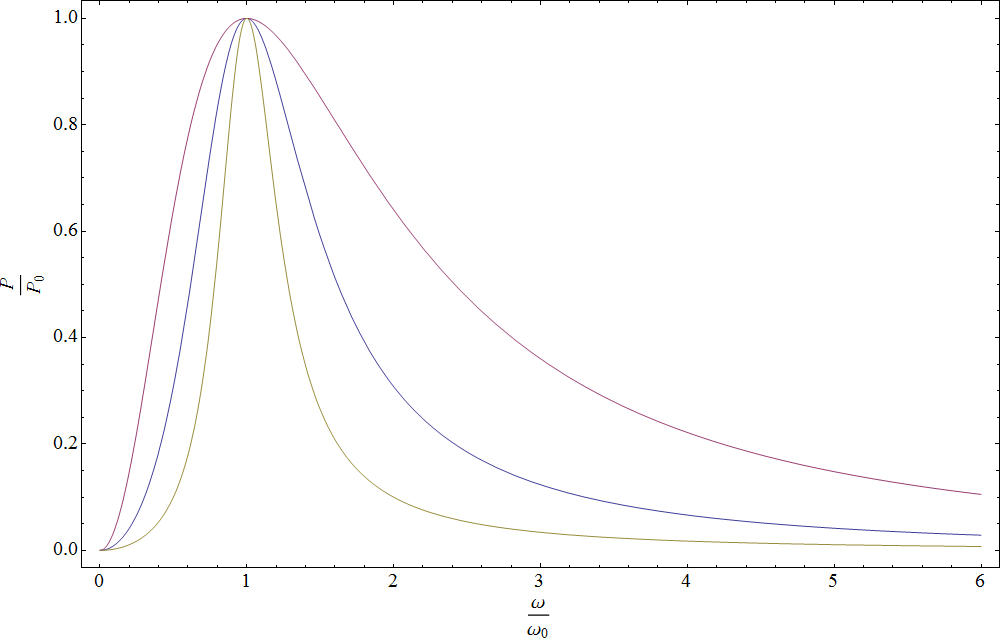
\includegraphics[scale=0.25]{resonancia}
		\caption{Gráfico de la potencia relativa en función de la frecuencia relativa, para diversas amortiguaciones. Cuanto menor amortiguación, más fina la curva}
		\label{fig:resonancia}
	\end{figure}
	y podemos ver que la frecuencia donde se obtiene la mitad de la potencia en resonancia, es decir semi-potencia, es 
	\begin{equation}
		\omega_{sp}^2 = \omega_0^2 \pm \gamma \omega
		\label{eq:oscilador_forzado_potencia_semipotencia}
	\end{equation}
	
\section{Oscilación con varios grados de libertad}
	En este apartado vamos a estudiar los sistemas con varios grados de libertad, enlazados con relaciones lineales, por lo que vale el principio de superposición. Como el sistema es lineal, la ecuación que vamos a resolver la podemos condensar en la siguiente relación (en coordenadas generalizadas)
    \begin{equation}
        \ddot{\vec{\psi}} = \sum_i C_i \psi_i = C_i \psi_i = A \vec{\psi}
        \label{eq:oscilador}
    \end{equation}
	y como son lineales tienen como soluciones una superposición o suma de soluciones armónicas, que denominamos modos normales
	\begin{equation}
		\vec{\psi}(t) = \sum_i c_i v_i e^{i (\omega_i t + \phi_i)} =  \sum_i c_i v_i \sen(\omega t + \phi_i)
		\label{eq:oscilador_solucion}
	\end{equation}
	es decir un modo normal es una solución donde todas las partes se mueven a una frecuencia idéntica, con fase inicial igual u opuesta, pero con una relación de amplitud característica de cada modo. Para obtener la solución anterior tenemos que probar la solución $\vec{\psi}(t) = \textbf{c} e^{i \omega t}$, con lo que obtenemos
	\begin{equation}
		\omega^2 \textbf{c} = A \textbf{c}
		\label{eq:oscilador_autovalores}
	\end{equation}
	que es una ecuación de autovalores y autovectores que puede ser resuelta por los métodos del álgebra lineal. Las coordenadas que dejan diagonal al la matriz $A$, es decir que desacopla el sistema, se denominan coordenadas normales, y a veces es posible por simple inspección obtenerlas (resolviendo el problema más fácilmente).
	\subsection{Pulsaciones}
		Consideremos un sistema con dos modos de oscilación con frecuencias muy parecidas (aunque tiene validez exacta la fórmula posterior, no tiene mucha importancia física si no son parecidas) con sus partes en un caso general de oscilación, es decir que el movimiento es suma de ambos modos. En ese caso definimos la frecuencia de modulación como
		\begin{equation}
			\omega_{mod} = \frac{|\omega_1 - \omega_2|}{2}
			\label{eq:oscilador_pulsaciones_modulacion}
		\end{equation}
		y la frecuencia de portadora o promedio
		\begin{equation}
			\omega_p = \frac{\omega_1 + \omega_2}{2}
			\label{eq:oscilador_pulsaciones_portadora}
		\end{equation}
		Con esas dos frecuencias podemos reescribir de la siguiente forma el movimiento de cada parte (consideramos que la fase y la amplitud son iguales, en caso contrario simplemente cambia el valor de la amplitud, que pasa a ser $A_1 + A_2$)
		\begin{equation}
			\psi = A_{mod}(t) \sen(\omega_p t) = 2 A \sen(\omega_{mod} t) \sen(\omega_p t)
			\label{eq:oscilador_pulsaciones}
		\end{equation}
		La formula anterior tiene validez para cualquier señal suma de dos señales armónicas muy cercanas, y para darnos una idea de la forma, en la figura \ref{fig:pulsaciones} vemos un ejemplo de pulsaciones
		\begin{figure}[H]
			\centering
			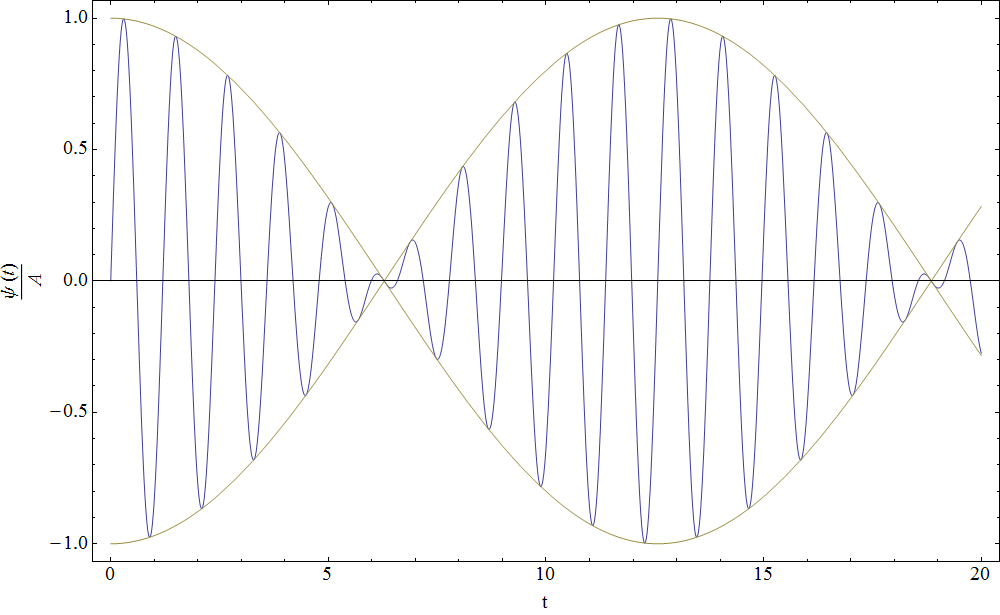
\includegraphics[scale=0.3]{pulsaciones}
			\caption{Pulsaciones producto de dos frecuencias diferenciadas en un 1\%, con portadora $\omega = 5$}
			\label{fig:pulsaciones}
		\end{figure}
\section{Oscilaciones de sistemas de muchos grados de libertad}
	  \label{sec:oscilador_recurrencia}
	  Al ir agrandando la cantidad de grados de libertad es necesario tener otro método para describir dicho sistema. El sistema general que usamos para describir el problema es
	  \begin{equation}
		\ddot{\psi_n} = c_{n-1} \psi_{n-1} + c_{n+1} \psi_{n+1} + c_n \psi_n
		\label{eq:oscilador_recurrencia}
	  \end{equation}
	  es decir lo definimos como una relación de recurrencia, independiente del elemento móvil elegido (se considera que todas las masas y los resortes son iguales, por simplicidad). Proponiendo como solución
	  \begin{equation}
		 \psi_n(t) = A_n \cos(\omega t - \phi)
		 \label{eq:oscilador_recurrencia_solucion}
	  \end{equation}
	  obtenemos una relación de recurrencia para las amplitudes
	  \begin{equation}
		 \omega^2 + c_n = \frac{c_{n-1} A_{n-1} + c_{n+1} A_{n+1}}{-A_n}
		 \label{eq:oscilador_recurrencia_relacion}
	   \end{equation}
	   Para la cual proponemos $A_n = \cos(k x_n) = \Re(e^{i k x_n})$, siendo $k = \frac{2 \pi}{\lambda}$ la frecuencia espacial o número de onda (y $\lambda$ la longitud de onda), obteniendo
	   \begin{equation}
			\frac{c_{n+1} e^{i k x_{n+1}} + c_{n-1} e^{i k x_{n-1}}}{-e^{i k x_n}} = \omega^2 + c_n
			\label{eq:oscilador_recurrencia_rel_dispersion}
	   \end{equation}
	   que es una relación entre la frecuencia temporal y la frecuencia espacial, lo que se denomina relación de dispersión. 
	   Luego hay que aplicarle condiciones de contorno al problema, es decir cuanto vale la coordenada $\psi_0$ y $\psi_N$ (siendo $N$ la cantidad de elementos), obteniendo el valor de frecuencia espacial y por lo tanto los modos de oscilación (frecuencias temporales) posibles.
\section{Ondas unidimensionales}
	    \subsection{Ondas estacionarias}
			Consideremos una cuerda de cuentas capaces de hacer oscilaciones transversales. Para describir ese sistema utilizamos el método de la sección \ref{sec:oscilador_recurrencia}, considerando pequeñas oscilaciones, por lo que la fuerza de la partícula $n$ es $\frac{- 2 T_0 \psi_n}{m a}$ (siendo $a$ la distancia inicial entre masas y $T_0 = k (a - l_0)$, la tensión inicial de cada resorte), entonces obtenemos la siguiente expresión
			\begin{equation*}
				\ddot{\psi}_n = \frac{T_0}{m a} (\psi_{n+1} + \psi_{n-1} - 2 \psi_n)
			\end{equation*}
			y la relación de dispersión será (considerando que $x_n = n a$)
			\begin{equation*}
				2 \cos(k a) = 2 \left(1 - 2 \sen^2\left(\frac{k a}{2}\right)\right) = 2 - \frac{m a}{T_0} \omega^2
			\end{equation*}
			es decir
			\begin{equation*}
				\omega^2 = \frac{4 T_0}{m a} \sen^2\left(\frac{k a}{2}\right)
			\end{equation*}
			si tomamos el límite con $N \to \infty$ y $a \to 0$, encontramos que $\psi_n(t) \to \psi(x,t)$, mientras $\psi_{n+1}(t) \to \psi(z + a,t)$ y $\psi_{n-1}(t) \to \psi(z - a,t)$. La ecuación diferencial del problema queda
			\begin{equation*}
				\partial_{tt} \psi(x,t) = \frac{T_0}{m a} (\psi(x+a,t) - 2 \psi(x,t) + \psi(x-a,t) = \frac{T_0 a}{m} \partial_{xx} \psi(x,t)
			\end{equation*}
			expresión que encontramos expandiendo en serie las funciones en $x +a$ y $x-a$. Observemos que la relación de dispersión queda
			\begin{equation*}
				\omega^2 = \frac{4 T_0}{m a} \sen^2\left(\frac{k a}{2}\right) \approx \frac{4 T_0}{m a} \left(\frac{k a}{2}\right)^2 = \frac{T_0 a k^2}{m}
			\end{equation*}
			es decir que la relación de dispersión indica que la frecuencia espacial es proporcional a frecuencia temporal o número de onda.
			
			La ecuación que quedó se denomina ecuación de onda clásica, y en general la escribimos de la siguiente forma
			\begin{equation}
				\frac{\partial^2 \psi(x,t)}{\partial t^2} = c^2 \frac{\partial^2 \psi(x,t)}{\partial x^2} \qquad \partial_{tt} \psi(x,t) = c^2 \partial_{xx} \psi(x,t)
				\label{eq:ondas_ecuacion}
			\end{equation}
			donde $c^2$ es la velocidad de propagación de la onda en el medio (que para un la cuerda es $c^2 = \dfrac{T_0}{\rho}$, siendo $\rho$ la densidad lineal de masa), que se relaciona con la siguente relación de dispersión
			\begin{equation}
				\omega = c\;k
				\label{eq:onda_dispersion}
			\end{equation}
			Para obtener una solución para esta ecuación de onda proponemos $\psi(x,t) = A(x) \sin(\omega t + \phi)$, por lo que obtenemos la siguiente ecuación
			\begin{equation*}
				\frac{d^2 A(x)}{d x^2} + \frac{\omega^2}{c^2} A(x) = A''(x) + k^2 A(x) = 0
			\end{equation*}
			que sabemos resolver, lo que obtenemos como solución general una superposición de soluciones oscilatorias
			\begin{equation}
				\psi(x,t) = \sum_{i,j} (c_i \sen(k_i x) + c_j \cos(k_j x)) \sen(\omega t + \phi)
				\label{eq:onda_solucion}
			\end{equation}
			y cada constante $c_i$ va a depender de las condiciones de contorno del problema, además de los modos posibles (es decir los valores posibles de $k$ y $\omega$). Esta ecuación corresponde a ondas estacionarias, nombre que tendrá sentido cuando observemos las ondas propagantes.
			
			Para condiciones iniciales tenemos que descomponer la función de la forma inicial en las componentes obtenidos de la solución \ref{eq:onda_solucion}, por medio de las series de Fourier, es decir
			\begin{equation}
				\psi(x,t) = \sum_{n=0}^{\infty} [(A_n \sen(n k_1 x) + B_n \cos(n k_1 x) ) \sen(\omega_n t + \phi)]
				\label{eq:onda_solucion_fourier}
			\end{equation}
			siendo $\omega_n = c k_n$ (la relación de dispersión de la ecuación de onda) y $A_n$ y $B_n$
			\begin{equation}
				A_n = \frac{1}{\tau} \int_{a}^{a + \tau} \psi(x,0) \sen\left(\frac{2 n\pi}{\tau} x\right) dx \qquad B_n = \frac{1}{\tau} \int_{a}^{a + \tau} \psi(x,0) \cos\left(\frac{2 n \pi}{\tau} x\right) dx
			\end{equation}
			mientras $B_0$ es
			\begin{equation}
				B_0  = \frac{1}{\tau} \int_{a}^{a + \tau} \psi(x,0) dx
			\end{equation}
			La constante $\tau$ representa la periodicidad de la función $\psi(x,0)$, que vendrá definido por el tamaño del problema físico (para una cuerda en general será $L$ o $2L$, siendo $L$ el largo de la cuerda), y $a$ es donde empieza el sistema físico, que en general se puede disponer que $a = 0$. También podemos escribir la serie de Fourier de forma exponencial, es decir
			\begin{equation}
				\psi(x,t) = \sum_{n=-\infty}^{\infty} C_n e^{i \frac{2 n \pi}{\tau} x} \sen(\omega_n t + \phi)
				\label{eq:onda_solucion_fourier_exp}
			\end{equation}
			
			Como todo problema mecánico, vamos a describir la energía de la onda estacionaria. La energía la tenemos que pensar como una densidad, es decir que se deriva de una integral sobre la coordenada espacial. La energía cinética la podemos encontrar como
			\begin{equation}
				T = \frac{1}{2} \int \rho \; (\partial_t \psi(x,t))^2 dx
				\label{eq:ondas_cinetica}
			\end{equation}
			siendo $\rho$ la densidad de masa lineal (ya que $\rho dx = dm$), o lo que corresponda dependiendo del caso, y la energía potencial podemos verla como 
			\begin{equation}
				V = \frac{1}{2} \int \lambda \; (\partial_x \psi(x,t))^2 dx
				\label{eq:ondas_potencial}
			\end{equation}
			siendo para una cuerda libre la constante $\lambda = T_0$ (la tensión de la cuerda). En la sección \ref{sec:ondas_reflexion} analizaremos el caso de la onda reflejada, por medio de un argumento físico y la energía de una onda propagante que, como veremos en la sección \ref{sec:ondas_propagantes}, es una solución más general de la ecuación de ondas
			%Propongamos, por simplificad, que $\psi(x,t) = A \cos(k x) \cos(\omega t)$, sin fase inicial en el espacio ni el tiempo (que es un caso simplificado de la solución general. De esta forma la energía nos queda	\[E = T + V = \frac{1}{2} A^2 \left(\int \rho \omega^2 \cos^2(k x) \sen^2(\omega t) dx + \int T_0 k^2 \sen^2(k x) \cos^2(\omega t) dx\right) = \frac{1}{2} A^2 \rho k^2 c^2 \left(\frac{x}{2} 
		\subsection{Ondas propagantes}
			\label{sec:ondas_propagantes}
			Existe una solución más general a la ecuación de ondas clásicas (ecuación \ref{eq:ondas_ecuacion}), que contempla una solución estacionaria (ondas estacionarias) en medios de propagación limitados y una solución propagante. Dicha solución es la siguiente
			\begin{equation}
				\psi(x,t) = \psi_1(x - c t) + \psi_2(x + c t)
				\label{eq:ondas_propagante}
			\end{equation}
			donde $\psi_1$ avanza en $x$ con el tiempo y $\psi_2$ retrocede. El perfil de la onda va a depender de la función inicial, pero en general vamos a trabajar con soluciones armónicas, es decir
			\begin{equation}
				\psi(x,t) = \Re\left(A e^{i (-k x + \omega t)} + B e^{i (k x + \omega t)}\right) = A \cos(\omega t - k x) + B \cos(\omega t + k x)
				\label{eq:ondas_propagante_armonica}
			\end{equation}
			
			Veamos que pasa con la expresión de la energía (ecuaciones \ref{eq:ondas_cinetica} y \ref{eq:ondas_potencial}) con la solución general \ref{eq:ondas_propagante} 
			\[E = T +  V = \frac{1}{2} \int \rho c^2 (\psi'_1 - \psi'_2)^2 dx + \frac{1}{2} \int \lambda (\psi'_1 + \psi'_2)^2 dx.\] Consideremos que $\psi_2 = 0$, es decir que tenemos solo propagación para un setido y que la propagación es armónica, entonces queda 
			\begin{equation}
				E(x,t) = \frac{1}{2} \Re(A) \left( \int \rho \omega^2 \Re\left(e^{i (-k x + \omega t)}\right)^2 dx - \int \lambda k^2 \Re\left(e^{i (-k x + \omega t)}\right) dx \right) = \frac{1}{2} \left(\frac{\rho \omega^2}{2k}-\frac{\lambda k^2}{2k}\right) \Re(A) \sen(2(-kx + \omega t))
			\end{equation}
			donde vemos que la energía avanza en el tiempo siguendo una forma armónica, contrario a lo que observamos en las ondas estacionarias (la solución con una onda propagandose para un sentido y para otro).
			
		\subsection{Reflexión de ondas}
			\label{sec:ondas_reflexion}
			Teniendo una solución propagante armónica \ref{eq:ondas_propagante_armonica} y un cambio repentino de medio (que se puede lograr en una cuerda cambiando la densidad) se genera un proceso de reflexión y transmisión de la onda propagante.
			
			Dispongamos el cambio de medio de $x = 0$, en ese punto pedimos que la continuidad de las soluciones de la ecuación de onda, que implica que la coordenada y su derivada espacial valgan lo mismo, es decir
			\begin{equation*}
				\psi_1(x = 0,t) = \psi_2(x = 0,t) \qquad \partial_x \psi_1(x = 0,t) = \partial_x \psi_2(x = 0, t)
			\end{equation*}
			y consideramos que tenemos un número de ondas para cada medio, es decir $k_1$ y $k_2$. De esta forma encontramos que
			\begin{align*}
				\psi_1(0,t) = (A + B) e^{i\omega t} = \psi_2(0,t) = C e^{i\omega t} \qquad &\Rightarrow \qquad A + B = C\\
				\partial_x \psi_1(0,t) =  i k_1 (B - A) = \partial_x \psi_2(0,t) = i k_2 C \qquad &\Rightarrow \qquad A + B = \frac{k_2}{k_1} C
			\end{align*}
			con lo que obtenemos que
			\begin{equation}
				B = \frac{k_1 - k_2}{k_1 + k_2} A \qquad C = \frac{2 k_1}{k_2 + k_1} A
				\label{eq:ondas_reflexion_amplitudes}
			\end{equation}
			y definimos coeficientes de transmición y reflexión de la siguiente manera
			\begin{equation}
				T = \frac{C}{A} = \frac{2 k_1}{k_1 + k_2} \qquad R = \frac{B}{A} = \frac{k_1 - k_2}{k_1 + k_2}
				\label{eq:ondas_reflexion_coeficientes}
			\end{equation}
			con lo que observamos que si $k_1 = k_2$ no hay reflexión, como es esperable, y la transmisión es total. Si el coeficiente $R = -1$, entonces $T = 0$ (observar que se verifica que $T - R = 1$), por lo que toda la señal es reflejada (que es el caso de ondas estacionarias). Estos coeficientes no dependen de la fase o la frecuencia de la onda incidente y además siempre van a ser reales, por lo que la reflexión y transmisión tendrá la misma fase inicial.
			En este contexto aprovechamos para definir la impedancia, que en general se define así
			\begin{equation}
				Z = \frac{F}{\partial_t \psi}
				\label{eq:ondas_reflexion_impedancia}
			\end{equation}
			es decir es la relación entre la fuerza o razón dinámica del movimiento (en una cuerda es la fuerza transversal) y el cambio de la coordenada generalizada. En una cuerda la impedancia tiene un valor definido $Z = \sqrt{T_0 \rho}$. En general la impedancia de un sistema es compleja, la parte real se denomina resistencia (determina el valor de la respuesta) y la parte imaginaria, reactancia (cambia la fase de la respuesta).
			
			Con esta magnitud definida podemos reescribir los coeficientes de transmisión y reflexión de la siguiente forma
			\begin{equation}
				R = \frac{Z_1 - Z_2}{Z_1 + Z_2} \qquad T = \frac{2 Z_1}{Z_1 + Z_2}
				\label{eq:ondas_reflexion_coeficientes_impedancia}
			\end{equation}
			ya que $Z = \frac{T_0}{c} = T_0 \frac{k}{\omega}$. Nuevamente vemos que no cambia la fase al reflejarse, y que si $Z_1 = Z_2$ la reflexión es nula (lo que se llama terminación perfecta).
			
			Como ya mencionamos si la reflexión es total estamos en un caso de onda estacionaria. En este caso no existe transmisión, por lo que toda la energía que llega al borde debe ser devuelta (ya que si no el borde cambiaría su estado dinámico, empezando a acelerar) y por lo tanto en una onda estacionaria no hay flujo neto de energía (toda la energía que vino de la fuente vuelve a la fuente).
			% Veamos otro caso, una cuerda con una masa $m$ en $x = 0$. Para poder resolver este problema tenemos que considerar la fuerza sobre la masa
			% \begin{equation*}
				% F = - T_0 \; \partial_x \psi_1 + T_0 \; \partial_x \psi_2 = m \; \partial_{tt} \psi_2
			% \end{equation*}
			% y sabiendo la expresión de $R$ y $T$ obtenemos
			% \begin{equation*}
				% i T_0 (k_1(1 - R) - k_2 T) = -m \omega^2 T
			% \end{equation*}
			% con lo que obtenemos
		\subsection{Paquetes de ondas}
			Veamos como se mueven dos ondas armónicas, propagandose para el mismo sentido, con frecuencias muy parecidas, es decir que la pertubación será
			\begin{equation*}
				\psi(x,t) = A e^{i(\omega_1 t - k_1 x)} + B e^{i(\omega_2 t - k_2 x)}
			\end{equation*}
			Para eso definimos la frecuencias promedios y las desviaciones
			\begin{equation}
				\omega = \frac{\omega_1 + \omega_2}{2} \quad \Delta \omega = \frac{\omega_1 - \omega_2}{2} \qquad k = \frac{k_1 + k_2}{2} \quad \Delta k = \frac{k_1 - k_2}{2}
				\label{eq:ondas_paquetes_batidos_frecuencias}
			\end{equation}
			por lo que la pertubación queda
			\begin{equation}
				\psi(x,t) = (A + B) e^{i (\omega t - k x)} \left(e^{i(\Delta \omega t - \Delta k x)} + e^{-i(\Delta \omega t - \Delta k x)}\right) = (A + B) e^{i(\omega t - k x)} \cos(\Delta \omega t - \Delta k x)
				\label{eq:ondas_paquetes_batidos}
			\end{equation}
			es decir que se da una pulsación de la ampltidud de la perturbación con frecuencia $\omega$ y $k$. 
			
			La velocidad de cada una de estas componentes es igual a $c = \frac{\omega}{k}$. En ese caso la velocidad del paquete modulante, que denominamos velocidad de grupo, es
			\begin{equation}
				c_g = \frac{\omega_1 - \omega_2}{k_1 - k_2} = \frac{\Delta \omega}{\Delta k} = \frac{d \omega}{d k}.
				\label{eq:ondas_paquetes_velocidad_grupo}
			\end{equation}
			Si las perturbaciones se mueven a diferentes velocidades entonces (ya que la relación de dispersión no es lineal) la modulación se va deformando con el tiempo, además que la velocidad de grupo puede ser más rápida o más lenta que la velocidad de fase. Para ver eso consideremos que la velocidad de grupo es una función del número de onda o la frecuencia angular, es decir
			\[ c_g = c_g(\omega) = c_g(k) \quad \Rightarrow \quad \Delta c_g = c_g(k) - c_g(k_0) = \left.\frac{d c_g}{d k}\right|_{k_0} \Delta k = \left.\frac{d^2 \omega}{d k^2}\right|_{k_0}  \Delta k\]
			por lo tanto la diferencia espacial es
			\[ \Delta x = x - x(t=0) = \left.\Delta x\right|_{t = 0} + \Delta c_g t\]
			es decir que si la velocidad de grupo cambia la frecuencia espacial o temporal el paquete se va deformando con el paso del tiempo.
			
			La ecuación de onda que permite que suceda este evento se denomina dispersiva, ya que el paquete de onda se va deformando en el tiempo.
			
			Ahora pasamos a describir una perfil de onda general, o paquete de onda, por medio del análisis de Fourier. Un perfil de onda físicamente posible (que sea continuo y que tenga longitud mucho menor que el medio de propagación) se puede descomponer en una base del espacio (en este caso vamos a utilizar exponenciales $e^{i \omega t}$ o $e^{i k x}$)
			\begin{equation}
				\psi(x,t) = \frac{1}{2\pi} \int_{-\infty}^{\infty}\int_{-\infty}^{\infty} A(\omega) B(k) e^{i(k x - \omega t)} d\omega dk = \mathcal{F}^{-1}[\hat{\psi}(k,t)] \mathcal{F}^-1[\hat{\psi}(x,\omega)]
				\label{eq:ondas_paquetes_fourier_general}
			\end{equation}
			donde definimos la transformada de Fourier $\mathcal{F}$ y su inversa $\mathcal{F}^{-1}$ de la siguiente forma
			\begin{equation}
				f(t) = \frac{1}{\sqrt{2 \pi}} \int_{-\infty}^{\infty} \hat{f}(\omega) e^{i \omega t} d\omega \qquad \hat{f}(\omega) = \frac{1}{\sqrt{2 \pi}} \int_{-\infty}^{\infty} f(t) e^{i \omega t} dt
				\label{eq:ondas_paquetes_fourier_def}
			\end{equation}
			donde llamamos espectro a la función $\hat{f}$. 
			
			Podemos usar tablas de transformadas para encontrarlas, ya que una la transformada es lineal, y también verifica algunas propiedades más interesantes (ver apéndice). Una propiedad muy importante es la relación entre el ancho de banda en frecuencia y en tiempo (o en frecuencia espacial y la posición), que determina una relación de incerteza; una señal muy definida en frecuencia no va a estar definida en tiempo, como por ejemplo una delta de Dirac 
			\[\delta(x) = \begin{cases} \infty & x = 0 \\ 0 & x \neq 0 \end{cases} \qquad \Rightarrow \qquad \displaystyle \int_{-\infty}^{\infty} \delta(x) f(x) dx = f(0)\]
			tiene una transformada igual una señal armónica, que no está definida en frecuencia espacial (vale lo mismo para tiempo o haciendo la antitransformada). La relación general que se encuentra es
			\begin{equation}
				\Delta x \Delta k \geq \frac{1}{2}
				\label{eq:ondas_paquetes_incerteza}
			\end{equation}
			que determina la dispersión espacial (o temporal) conociendo la dispresión en frecuencia (o ancho de banda) y visceversa. Es una relación fundamental que mantiene la información entre transformaciones hechas.
\section{Ondas especiales}
	El análisis hecho hasta ahora, en general, asumió perturbaciones que son solución de la ecuación de onda clásica. Ahora vamos a analizar un caso particular donde la ecuación de ondas no es la clásica y además es dispersiva. 
	
	Consideremos $N$ péndulos con misma masa acoplados con resortes de constante $k$. Hacemos el análisis dinámico (aplicado las leyes de Newton) considerando que el número $N$ es muy grande (así como se hizo en la sección \ref{sec:oscilador_recurrencia}).
	\[ m \ddot{\psi}_n = - \frac{m g}{l} \psi_n + k (\psi_{n+1} - \psi_n) - k ( \psi_n - \psi_{n+1}) \]
	y si hacemos el pasaje al continuo obtenemos \[\psi_{n+1} \to \psi(x + a, t) = \psi(x, t) + a \partial_x \psi + a^2 \partial_{xx} \psi\] y lo mismo para $\psi_{n-1}$, con lo que obtenemos
	\begin{equation}
		\partial_{tt} \psi(x,t) = - \omega_0^2 \psi(x,t) + \frac{K a^2}{m} \partial_{xx} \psi(x,t)
		\label{eq:ondas_klein_gordon}
	\end{equation}
	que se denomina ecuación, de ondas, de Klein-Gordon. Si proponemos la solución $\psi(x,t) = A(x) e^{i (\omega t + \phi)}$ obtenemos
	\[ \frac{k a^2}{m} \frac{d^2 A}{d z} - (\omega_0^2 - \omega^2)A(z) = 0\]
	ecuación que tiene solución exponencial pura (solución que decimos está en la zona reactiva) para $\omega > \omega_0$ y una solución armónica para $\omega < \omega_0$ (decimos que es la zona activa). 
	
	Para encontrar la relación de dispersión propongamos una solución al caso discreto y luego hagamos el paso al límite continuo. Si proponemos $\psi_n = A_n e^{i \omega t}$, obtenemos la relación \[m \omega^2 A_n = \frac{m g}{l} A_n - K (A_{n+1} + A_{n-1} - 2 A_n),\] para la cual proponemos $A_n = A e^{i k a n}$, con lo que nos queda \[m \omega^2 = \frac{m g}{l} + 4 K \sen^2\left(\frac{k a}{2}\right)\] que en el límite nos queda
	\begin{equation}
		\omega^2 = \frac{g}{l} + \frac{K a^2}{m} k^2 = \omega_0^2 + c^2 k^2
		\label{eq:ondas_klein_gordon_dispersion}
	\end{equation}
	es decir que que existe una dispersión, ya que $k \neq c^{-1} \omega$.
\section{Ondas en varias dimensiones}
	Para generalizar escribimos, de forma natural, la ecuación de ondas clásica en el espacio euclidio.
	\begin{equation}
		\nabla^2 \psi(\textbf{r},t) = \frac{1}{c^2} \partial_{tt} \psi(\textbf{r},t)
		\label{eq:ondas_ecuacion_general}
	\end{equation}
	donde el operador $\nabla^2$ se denomina laplaciano y vale
	\begin{equation}
		\nabla^2 = \partial_{xx} + \partial_{yy} + \partial_{zz}
		\label{eq:laplaciano_cartesianas}
	\end{equation}
	La solución que vamos a manejar corresponde a la propagación de una onda en un sentido (fuera de la fuente) con perfil armónico, es decir
	\begin{equation}
		\psi(\textbf{r},t) = A(\textbf{r}) e^{i (\textbf{k} \cdot \textbf{r} - \omega t)}
		\label{eq:ondas_ecuacion_general_solucion}
	\end{equation}
	donde el numero de onda $k$ pasa a ser un vector que determina la dirección de propagación de la onda, cuyo modulo sigue verifcando la relación de dispersión. De esa forma podemos tener varios frentes de ondas posibles, siendo un frente de onda la región del espacio con la misma fase a un mismo tiempo (es decir la región del espacio que verifica $\textbf{k} \cdot \textbf{r} = \text{cte}$). 
	
	Si tenemos una fuente puntual el frente de onda será esférico podemos ensayar en la ecuación de ondas la siguiente solución, que es isotrópica, \[\psi(\textbf{r},t) = f(r) e^{i (\omega t - k r)}\] con lo que obtenemos \[\frac{df}{dr} + \frac{f}{r} = 0\] que tiene por solución
	\begin{equation}
		A(\textbf{r}) = \frac{A}{r}
		\label{eq:ondas_ecuacion_general_amplitud_esferica}
	\end{equation}
	es decir que la amplitud decae con la distancia como una homográfica. La intensidad de la onda la podemos encontrar como el cuadrado de la amplitud, por lo que la intensidad de cae como $r^{-2}$, como es de esperar ya que la superficie de una esfera de propoprcional al radio cuadrado.
	
	Podemos hacer el mismo análisis para una fuente cilindrica, pero es más complejo, por lo que presentamos la solución final
	\begin{equation}
		A(\textbf{r}) = \frac{A}{\sqrt{\rho}}.
		\label{eq:ondas_ecuacion_general_amplitud_cilindrica}
	\end{equation}
	Finalmente un fente de onda plano tiene la siguiente amplitud
	\begin{equation}
		A(\textbf{r}) = A
		\label{eq:ondas_ecuacion_general_amplitud_plana}
	\end{equation}
	es decir un fente de onda plano mantiene la amplitud
	\subsection{Reflexión de ondas planas}
		Consideremos que una onda plana incide en una superficie plana interfaz de dos medios con diferentes velocidades de propagación (en este punto la onda plana ayuda al análisis simplificado pero las ecuaciones tienen validez general). El $\textbf{k}$ está contenido en el plano xz y la interfaz está dispuesta en el eje $z = 0$, lo que nos permite resolver el problema ayudandonos de la simetría.
		
		La onda incidente tiene la siguiente forma (considerando que no se desplaza en el eje $y$) \[ \psi(x,y,z,t) = A e^{i (\omega t - k_x x - k_z z)}\] y en el punto $z = 0$ valdrá \[\psi(x,y,z=0,t) = A e^{i(\omega t - k_x x)}\] como esperabamos. Sabemos que $k^2 = k_x^2 + k_y^2 + k_z^2$, por lo que $k_z = \pm \sqrt{k^2 - k_x^2 - k_y^2}$, es decir existe dos posibles rayos que verifican la relación en $z = 0$, una es la incidente y otra es la reflejada. La onda reflejada se propaga con el mismo $k_x$ y $k_z$ con signo cambiado, por lo que tiene el mismo ángulo respecto a la normal al plano, es decir
		\begin{equation}
			\theta_i = \theta_r
			\label{eq:ondas_reflexion_ley}
		\end{equation}
		ecuación que se conoce con la ley de reflexión especular.
		
		Consideremos que la onda transmitida sufre un cambio en su amplitud dependiendo de un coeficiente de transmisión $T$ independiente de la posición o del tiempo, el cual va a depende finalmente de la física de la interfaz y la onda. Además que por continuidad el número de ondas en el eje x debe ser igual de ambos lados. Es decir que la señal transmitida será \[ \psi_t(x,y,0,t) = A T e^{i (\omega t - k_{i_x} x)} = B e^{i(\omega t - k_{2_x})}\]
		lo que nos lleva a que 
		\begin{equation}
			k_{1_x} = k_{2_x} = k_1 \sen(\theta_i) = k_2 \sen(\theta_t) = n_1 \sen(\theta_i) = n_2 \sen(\theta_t)
			\label{eq:ondas_transmision_snell}
		\end{equation}
		donde definimos $n_i = \frac{c k_i}{\omega} = \frac{c_i}{c}$ como el indice de refracción.
\section{Óptica geométrica}
		Esta óptica es estudio de elementos ópticos solo con consideraciones geometricas (ya que podemos despreciar la longitud de onda $\lambda$ de la onda). En esta sección vamos a analizar como alterar frentes de ondas por medio de elementos refractantes y reflectantes, despreciando efectos físicos de la onda (ver \ref{sec:difraccion}).
		
		Para este estudio riguroso vamos a usar dos principios de gran importancia no solamente en la óptica sino también en otras ramas. Primeramente, tenemos el principio de Huygens (que después vamos a completar y formalizar en la sección \ref{sec:difraccion}) que determina que cada frente de onda lo podemos describir como una sucesión de fuentes esféricas (con las mismas frecuencias que el frente) que generan la envolvente del frente; este principio tiene algunas limitaciones, pero se puede probar que es una consecuencias de la ecuación de onda. El segundo principio que vamos a utilizar es un principio variacional (el primero, históricamente, utilizado), el principio de Fermat, que pregona que el camino óptico que finalmente recorre un haz en ir de un punto $A$ a un punto $B$ es la solución estacionaria respecto a variaciones de dicho y en general consideraremos el camino óptico mínimo (ya que no existe máximo). Este principio lo podemos escribir así
		\begin{equation}
			\delta S = \delta \int_{A}^{B} n(s) ds = 0
			\label{eq:optica_fermat}
		\end{equation}
		es decir que la variación de esa integral sea nula, por lo que el camino óptico (que podemos notar $S$ o $LCO$, dependiendo del contexto) es estacionario. El principio se puede utilizar para encontrar la ley de Snell, considerando que le tiempo que tarda de ir de un punto a otro es mínimo, es decir \[ t = \frac{\vec{AO}}{v_1} + \frac{\vec{OB}}{v_2} = \frac{\sqrt{h^2+x^2}}{v_1} + \frac{\sqrt{b^2+(a - x)^2}}{v_2}\] siendo $h$ la altura desde la interfaz al punto $A$, $x$ la distancia paralela a la interface del punto $A$ al punto de contacto, $b$ la altura desde la interfaz hasta el punto $B$ y $a$ la distancia paralela a la interfaz del punto $A$ al punto $B$. El único parametro es la distancia $x$, por lo que debemos derivar el tiempo respecto a dicho \[\frac{d t}{d x} = \frac{x}{v_1 \sqrt{h^2 + x^2}} + \frac{ -(a - x)}{v_2 \sqrt{b^2 + (a - x)^2}} = 0\] lo que finalmente queda (considerando que $n = \frac{c}{v_1}$).
		\begin{equation}
			n_1 \sen(\theta_1) = n_2 \sen(\theta_2)
			\label{eq:snell}
		\end{equation}
		la ley de Snell
	
	\subsection{Lentes}
		Una lente es un sistema óptico refractor, es decir un sistema con una discontinuidad en el indice de refracción respecto al medio, que varia la distribución de la energía incidente. Con esta definición podemos clasificar como lentes variados objetos en variados espectros de rayos (UV, IR, microondas y hasta sonido). En este curso vamos a analizar lentes esféricas, sin considerar lentes asfericas (que se pueden analizar por medio del principio de Fermat y la geometría analítica) ya que son de muy dificiles de producir.
		
		Analizemos un rayo que incide en una superfície esférica de radio $R$, el camino óptico que efectúa es \[LCO = n_1 l_o + n_2 l_i\] que podemos escribir utilizando el teorema del coseno de la siguiente manera \[LCO = n_1\sqrt{R^2 + (s_o + R)^2 - 2 R (s_o + R) \cos(\phi)} + n_2\sqrt{R^2 + (s_i - R)^2 - 2 R (s_i - R) \cos(\phi)},\] siendo $s_o$ la distancia entre el vertice (el punto más cercano al objeto, por donde pasa el eje óptico de la superficie) y la fuente, llamado distancia objeto, mientras que $s_i$ es la distancia imagen, donde se une el eje óptico y el haz refractado. El ángulo $\phi$ es el ángulo del radio vector del punto de incidencia del haz, que va a ser el parametro del camino óptico, es decir que vamos a hacer $\frac{d LCO}{d\phi} = 0$ lo que nos queda 
		\[\frac{n_1 R (s_o + R) \sen(\phi)}{2 l_0} - \frac{n_2 R (s_i - R) \sen(\phi)}{2 l_i} = 0 \qquad \Rightarrow \qquad \frac{n_1}{l_o} + \frac{n_2}{l_i} = \frac{1}{R}(\frac{n_2 s_i}{l_i} - \frac{n_1 s_o}{l_o}.\] 
		Esta expresión es muy complicada de llevar a la práctica, por lo que se hace una aproximación a primer orden, que corresponde con $\sen(\phi) \approx \phi$ y los rayos son paraxiales, es decir $l_x = s_x$ para imagen y objeto, lo que se llama óptica gaussiana. De esta forma nos queda
		\begin{equation}
			\frac{n_1}{s_o} + \frac{n_2}{s_i} = \frac{n_2 - n_2}{R}
			\label{eq:lentes_esferica}
		\end{equation}
		Podemos definir dos distancias importantes, denominadas foco objeto y foco imagen, que corresponden al punto donde el frente de onda converge en o del infinito respectivamente (es decir que el foco objeto corresponde a la distancia objeto donde el frente de onda en la lente es plano y el foco imagen corresponde a la distancia imagen que se forma al tener una un frente de onda plano incidente). Por lo tanto siguien la siguiente relación 
		\begin{equation}
			 f_o = \frac{n_1}{n_2 - n_1} R \qquad f_i = \frac{n_2}{n_2 - n_1} R
			 \label{eq:lentes_foco_objeto_imagen}
		\end{equation}
		
		Otra clasificación importante es objeto e imagen virtual o real. Un objeto es real cuando los rayos convergen del objeto, mientras que es virtual si los rayos convergen hacia el. Lo contrario pasa para la imagen. En nuestra convención, la más usual en óptica geométrica, las distancias objeto e imagen son positivas si son reales (lo mismo aplica para el foco) y negativa si son virtuales.
		
		Las lentes que vamos a analizar ahora son de dobre interfaz, en general dos indices de refracción, el del medio y el de la lente. La imagen de la primera interfaz va a pasar ser el objeto de la segunda interfaz, por lo que podemos considerar que $|s_{o_2}| = |s_{i_2}| + d$, siendo $d$ el espesor de la lente entre vertices, y considerando la convención propuesta obtenemos $s_{o_2} = - s_{i_1} + d$ por lo que al sumar la relación \ref{eq:lentes_esferica} para ambas interfaces obtenemos
		\begin{equation}
			n_{e} \left(\frac{1}{s_{o_1}} + \frac{1}{s_{i_2}}\right) = (n_l - n_e)\left(\frac{1}{R_1} - \frac{1}{R_2}\right) + \frac{n_l d}{(s_{i_1} - d) s_{i_1}}
			\label{eq:lentes_general}
		\end{equation}
		y si despreciamos el valor $d$, es decir consideramos lentes delgadas, nos queda (considerando que las distancias son las mismas medidas desde cualquier vértice)
		\begin{equation}
			\frac{1}{s_o} + \frac{1}{s_i} = \frac{(n_l - n_e)}{n_e} \left(\frac{1}{R_1} + \frac{1}{R_2}\right)
			\label{eq:lentes_constructores}
		\end{equation}
		y podemos deducir que el foco imagen y foco objeto son iguales, por lo que obtenemos que
		\begin{equation}
			\frac{1}{s_o} + \frac{1}{s_i} = \frac{1}{f}
			\label{eq:lentes_guassiana}
		\end{equation}
		denominada fórmula gaussiana para lentes delgadas.
		
		Consideremos un objeto de extensión finita, que por abstraccion lo vemos como un conjunto infinito de puntos. De un gráfico podemos deducir, considerando que la altura debajo del eje óptico es negativa, que
		\begin{equation}
			M_T = \frac{y_o}{y_i} = -\frac{s_i}{s_o}
			\label{eq:lentes_aumento_transversal}
		\end{equation}
		que es el aumento transversal de la imagen. Con un poco de trabajo algebraico podemos llegar a la formula newtoneana
		\begin{equation}
			x_o x_i = f^2
			\label{eq:lentes_newton}
		\end{equation}
		donde $x$ es la distancia del objeto o imagen al foco (donde queda evidente, considerando la convención, que como el $f^2$ es siempre positivo, la imagen y el objeto deben estar opuestos respecto al respectivo punto focal). El aumento lateral o longitudinal de una lente se define y vale lo siguiente
		\begin{equation}
			M_L = \frac{d x_i}{d x_o} = - \frac{f^2}{x_0^2} = - M_T
			\label{eq:lentes_aumento_lateral}
		\end{equation}
		es decir que si la imagen está derecha los objetos parecen más cerca de lo que realmente están, que es lo que se logra con una lupa por ejemplo.
		
		\subsection{Espejos}
		Un espejo es un elemento puramente reflector, para el cual vamos a estudiar únicamente con la ley de reflexión \ref{eq:ondas_reflexion_ley}. La aproximación que vamos a tomar es que no absorben nada de la radiación incidente, es decir son espejos perfectos. 
		
		Analizar un espejo plano es una tarea muy sencilla, ya que lo único que hace es reflejar perfectamente sin alterar la imagen más que por un giro o inversión de los sentidos (observable en un simple trazado de rayos). De esta forma vamos a analizar espejos esféricos (dejando los asfericos de lado, pero dichos son estudiables fácilmente con la ley de reflexión y geometría analítica). Veamos un espejo concavo, que por convención tiene radio negativo (ya que el centro de la superficie se haya a la izquierda del vertice). La imagen puntual (ya que el objeto utilizado es puntual, ubicado en $s_o$) que se va a generar es de origen real, por lo que será positiva (esta es la conveción utlizada también para lentes), cruzará el eje optico a una distancia $s_i$ del vertice. Considerando rayos paraxiales, es decir que la distancia entre el punto de contacto y la distancia objeto son aproximadamente iguales y lo mismo para la distancia imagen, podemos probar, por argumentos gráficos, que la siguiente expresión tiene validez
		\begin{equation}
			\frac{1}{s_o} + \frac{1}{s_i} = - \frac{2}{R}
			\label{eq:espejos_esfericos}
		\end{equation}
		y de donde deducimos que el foco es igual a
		\begin{equation}
			f_o = f_i = - \frac{R}{2}
			\label{eq:espejos_esfericos_foco}
		\end{equation}
		por lo que podemos deducir que
		\begin{equation}
		 \frac{1}{s_o} + \frac{1}{s_i} = \frac{1}{f}
		 \label{eq:espejos_esfericos_ecuacion}
		\end{equation}
		donde queda evidente que podemos utilizar todas las ecuaciones derivadas para las lentes delgadas por similitud matemática, considerando la convención de signos correspondiente.
		
		%FALTA PRISMAS
\section{Polarización}
	De las ecuaciones de Maxwell obtenemos que la onda electromagnética, la luz, es una onda vectorial transversal, es decir que es una onda con diferentes planos de oscilaciones posibles. En esta sección analizaremos que sucede cuando dos ondas linealmente polarizadas con fases diferentes son colineales, y por lo tanto se suman. Esto genera un cambio en el estado de polarización y veremos como se puede describir. 

	Para simplificar consideremos los campos eléctricos (ya que el campo magnético es perpendicular en los casos que vamos a tratar) están contenidos en un plano (que denominamos xy), es decir que en general \[ \textbf{E} = (\hat{x} E_x + \hat{y} E_y) e^{i(k z - \omega t)}\] donde $E_x$ e $E_y$ son magnitudes complejas que permite agregarle una fase a al campo en una coordenada. Si los $E_x$ e $E_y$ son reales, la polarización es claramente lineal, girada dependiendo del valor de cada campo. Mientras si $\displaystyle E_y = \|E_x\| e^{i \left(-\frac{pi}{2}\right)}$, obtenemos polarización circular (ya que $E_x^2 + E_y^2 = 1$) en este caso derecha (se vueve siguiendo las agujas de reloj respecto a la fuente) y si la fase es $\frac{pi}{2}$ obtenemos una polarización circular izquierda (para analizar esto rápidamente se debe ver como cambia el campo con el tiempo).
	
	El caso general es la polarización eliptica, que corresponde a una diferencia de fase en alguna componente y magnitud de componentes diferentes, es decir 
	\begin{align*}
		E_x &= \|E_x\| e^{i(k z - \omega t)}\\
		E_y &= \|E_y\| e^{i (k z - \omega t + \epsilon)}
	\end{align*}
	Podemos escribir la siguiente expresión, que se deduce facilmente (acá tomamos la parte real de la onda y utilizamos la identidad trigonométrica de la suma de ángulos) \[\frac{E_y}{\|E_y\|} - \frac{E_x}{\|E_x\|} \cos(\epsilon) = - \sen(k z - \omega t) \sen(\epsilon) = - \sqrt{1 - \frac{E_x}{\|E_x\|}} \sen(\epsilon)\]
	donde al final se hizo uso de la ecuación del campo en $x$ más la identidad trigonométrica de Pitágoras. Finalmente nos queda la siguiente expresión
	\begin{equation}
		\left(\frac{E_y}{\|E_y\|}\right)^2 + \left(\frac{E_x}{\|E_x\|}\right)^2 - 2 \left(\frac{E_y}{\|E_y\|}\right) \left(\frac{E_x}{\|E_x\|}\right) \cos(\epsilon) = \sen^2(\epsilon)
		\label{eq:polarizacion_elipitica}
	\end{equation}
	que tiene validez general (ya que para la polarización circular $\epsilon = \frac{pi}{2}$ y queda una circunferencia, mientras si es lineal $\epsilon = 0$ quedando una relación lineal). De la ecuación anterior obtenemos el ángulo del eje $x$ de la elipse respecto a la base 
	\begin{equation}
		tg(2\alpha) = \frac{2 \|E_x\| \|E_y\| \cos(\epsilon)}{\|E_x\|^2 - \|E_y\|^2}
		\label{eq:polarizacion_eliptica_angulo}
	\end{equation}
	
	La polarización de una fuente natural es un tema especial, ya que las fuente generan trenes de ondas con cierta longitud (que se denomina de coherencia) con una polarización definida por un tiempo determinado (tiempo de coherencia), por lo que la luz natural no tiene una polarización definida en el tiempo (denominada polarización al azar). Mientras un tren de ondas infinito, o una onda monocromática, debe estar siempre polarizado. La realidad física corresponde a ambas situaciones, lo que se denomina parcialmente polarizado.
	
	Ahora pasamos a describir los diferentes elementos capaces de cambiar la polarización de la luz incidente, denominados polarizadores. Analizemos primeramente un polarizador lineal, del que podemos deducir ,por medio de un esquema simple, que el campo eléctrico después del polarizador es \[E = E_0 \cos(\theta) \hat{n}\] donde $\hat{n}$ es la dirección en el plano xy del eje del polarizador, por lo que la intensidad a la salida será
	\begin{equation}
		I(\theta) = I(0) \cos^2(\theta)
		\label{eq:polarizacion_malus}
	\end{equation}
	que se denomina la ley de Malus. 
	
	Veamos algunos tipos de polarización por medio de elementos materiales, donde tenemos elementos dicroicos y bifringentes (lo que son polarizadores por transmisión). Un elemento dicroico es un material que absorbe una componente del campo eléctrico, por medio de una fuerte anisotropía de su estructura, y deja pasar la luz en un eje denominado óptico; ejemplos de elementos dicroicos son los cristales de turmalina, o las láminas polarizadoras lineales (llamadas polaroides). Un material bifringente exhibe anistropía en el indice de refracción, en general en dos ejes (uno óptico u ordinario y uno extraordinario), que permite que se generen dos imagenes; el funcionamiento de un elemento bifringente es idéntico a un material dicroico, separando de la luz que sale una componente del campo eléctrico.
	
	Luego tenemos la polarización por reflexión en medios dielétricos, para el cual tenemos que hacer un análisis de la dinámica del problema. Al incidir una onda electromagnetica con una polarización definida logramos que los dipolos moleculares se acomplen con dicha perturbación, obteniendo una onda reflejada. Si la onda es incide justamente con el campo eléctrico perpendicular al los dipolos no se reflejará onda alguna y todo será transmitido. Ese ángulo se denomina ángulo de Brewster y es fácilmente deducible sabiendo que $\theta_t + \theta_B = 90^\circ$ (ya que la onda transmitida va ser ortogonal a los dipolos del material)
	\begin{equation}
		\theta_B = \arctg\left(\frac{n_2}{n_1}\right)
		\label{eq:polarizacion_brewster}
	\end{equation}
	
	Finalmente nos queda un elemento óptico importante cuando se describe la polarización, los retardadores, que básicamente agregan una fase determinada a uno de los ejes (el eje rápido), cambiando la polarización de la onda incidente. Existen retardadores de media onda, onda completa y cuarto de onda que agregan una fase de, respectivamente, $2\pi$, $\pi$ y $\frac{\pi}{2}$ a la componente del eje rápido, pudiendo obtener a la salida una polarización eliptica, circular o lineal dependiedo de cada caso.
	
\section{Interferencia}
	\label{sec:interferencia}
	El proceso de interferencia consiste en la superposición de una o más ondas, y vamos a hacer hincapie en las ondas electromagnéticas (teniendo que considerar la naturaleza vectorial de las ondas). Para empezar el análisis consideremos dos fuentes puntuales monocromáticas separadas más de una longitud de onda (para despreciar efectos de difracción) y veamos como interaccionan en un punto lo suficientemente alejado (por distancia real o por medio de lentes) para que sea un frente plano. En ese punto el campo eléctrico será \[\textbf{E} = \textbf{E}_{1} + \textbf{E}_2 = \textbf{E}_{o_1} e^{i (\textbf{k}_1 \cdot \textbf{r} - \omega t + \epsilon_1)} + \textbf{E}_{o_2} e^{i (\textbf{k}_2 \cdot \textbf{r} - \omega t + \epsilon_2)}.\] Aca consideramos que las ondas tiene el mismo plano de polarización (y son linealmente polarizadas) para simplificar el análisis. Consideremos que la intensidad del campo eléctrico como el cuadrado de dicha magnitud vectorial, es decir \[E^2 = \textbf{E} \cdot \textbf{E} = \|\textbf{E}_1\|^2 + \|\textbf{E}_2\|^2 + 2 \textbf{E}_1 \cdot \textbf{E}_2 = I_1 + I_2 + 2 \textbf{E}_{o_1} \cdot \textbf{E}_{o_2} e^{i \omega t} e^{ i (\epsilon_1 + \epsilon_2)} e^{i (\textbf{k}_1 + \textbf{k}_2) \cdot \textbf{r}},\] y si consideramos el promedio temporal de la intensidad (lo que se llama irradiancia relativa) obtenemos que el termino final no depende del tiempo (ya que integramos en un periodo mucho más grande que $\dfrac{2\pi}{\omega}$) y que la irradiancia queda 
	\begin{equation}
		I = \langle\|\textbf{E}_1\|^2\rangle_T + \langle\|\textbf{E}_1\|^2\rangle_T + \textbf{E}_{o_1} \cdot \textbf{E}_{o_2} \cos((\textbf{k}_1 - \textbf{k}_2)\cdot \textbf{r} + \epsilon_1 - \epsilon_2)
		\label{eq:interferencia_general}
	\end{equation}
	y en el caso que los campos tengan el mismo plano de oscilación nos queda que
	\begin{equation}
		I = I_1 + I_2 + 2 \sqrt{I_1 I_2} \cos(\delta)
		\label{eq:interferencia_particular}
	\end{equation}
	donde $\delta$ representa la diferencia de camino óptico y de fase inicial de las ondas que se superponen. Un caso de mucha importancia practica es cuando las fuentes tienen la misma irradiancia, lo que terminamos obteniendo la siguiente expresión
	\begin{equation}
		I = 2 I_0 \cos^2\left(\frac{\delta}{2}\right)
		\label{eq:interferencia_patron_clasico}
	\end{equation}
	Los puntos donde la interferencia es máxima o minimia (llamada, respectivamente, destructiva o constructiva) forman una superficie que podemos encontrar de la siguiente forma (para un frente de onda esférico producto de una fuente puntual, considerando que la distancia es suficientemente grande para despreciar cambios de la amplitud)
	\begin{align}
		\delta = 2n\pi \qquad &\Rightarrow \qquad r_1 - r_2 = \frac{2n\pi + \epsilon}{k} = n\lambda + \frac{\epsilon}{k}\\
		\delta = (2n + 1)\pi \qquad &\Rightarrow \qquad r_1 - r_2 = \frac{(2n + 1)\pi + \epsilon}{k}
	\end{align}
	ecuaciones que corresponden hiperboloides de revolución.
	
	El análisis que hicimos acá corresponde a dos ondas de extensión infinita, la cual es generada por una fuente de forma continua. Pero en general las fuentes generan de forma intermitente, durante un tiempo determinado, que vamos a llamar tiempo de coherencia. La coherencia es la capacidad de interferir de forma correcta con dos fuentes, que se va a dar dependiendo solamente de las frecuencias temporales y la frecuencias espaciales (además de la polarización). Volviendo, el tiempo de coherencia va a determinar las componentes del paquete de onda, por lo que va a determinar qué tan pura va a ser el espectro y por lo tanto que tan visibles van a ser las franjas (ya que solo interfieren ondas de la misma frecuencia temporal, como ya vimos). La coherencia espacial, mientras tanto, determina cuanto varia en el tiempo la fase relativa entre dos puntos del espacio fijos, que va a venir determinado por la forma del frente de onda y la fuente. También la coherencia se da, para una onda vectorial como la luz, si la superposición comparten componentes de polarización, como vimos en la ecuación \ref{eq:interferencia_general}
	
	Existen varios tipos de interferómetros, que dividimos por el tipo de proceso físico que efectuan, división de frente de onda o división de amplitud. 
	
	El inteferómetro por división de frente de onda más común es el de Young, el cual consiste en una fuente coherente que pasa por dos ranuras muy estrechas. Haciendo el análisis geométrico, considerando la aproximación paraxial de los rayos obtenemos que la franjas están distanciadas
	\begin{equation}
		\Delta y = \frac{L}{d}\lambda
		\label{eq:interferencia_young_interfranja}
	\end{equation}
	que obtenemos sabiendo que la diferencia de camino óptico tiene que ser igual a $m\lambda$, lo que obtenemos que los máximos están en 
	\begin{equation}
		y_m = \frac{L}{d} m \lambda
		\label{eq:interferencia_young_maximos}
	\end{equation}
	y por lo tanto la irradiancia será
	\begin{equation}
		I = 4 I_o \cos^2\left(\frac{y d \pi}{L\lambda}\right)
		\label{eq:interferencia_young_irradiancia}
	\end{equation}
	
	Los demás interferómetros por división de frente de onda se puede reducir al interferómetro de Young, haciendo consideranciones respecto a las fases de las fuentes (ya que si se usa espejos la fase cambia en $\pi$ si es razante, es decir ángulo de incidencia mayor a 90$^\circ$). Podemos enumerar en estos interferómetros al espejo de Lloyd (donde se genera una fuente nueva con un espejo donde incide razante la fuente), el doble espejo de Fresnel (que son dos espejos planos que generan dos fuentes a partir de una, que terminar interfiriendo en una zona definida del espacio) o el biprisma de Fresnel (un primsa doble que genera una franja.
	
	Los interferómetros por división de amplitud consisten en dividir la onda en dos partes por medio de un espejo, y luego unirlas (generando una diferencia de camino óptico) en algún punto. Vamos a diferenciar interferómetros por reflexión pura o con refracción (estos últimos son creados por películas dieléctricas). 
	
	Analizaremos primeros los de refracción, que corresponde a la interferencia producto de una película dieléctrica. Parte de los haces (consideramos que son originarios de una fuente puntual coherente) son reflejadados además de transmitidos, por lo que analizando un haz incidente observamos un reflejado y luego un transmitdo que también será reflejado y que finalmente saldá con el mismo ángulo que incidió; si logramos con una lente converger el primer rayo y el segundo rayo reflejado tendremos franjas de interferencia dependientes de la diferencia de camino óptico, que finalmente depende del ángulo de incidencia (por lo que se llaman franjas de igual inclinación) de la siguiente manera
	\begin{equation}
		\Delta LCO = 2 n d \cos(\theta_t)
		\label{eq:interferencia_franjas_inclinacion}
	\end{equation}
	De esta forma es posible utilizar una fuente extensa para lograr franjas con la misma inclinación, siempre que se logre la coherencia temporal.
	
	El otro tipo de franjas se denomina de igual espesor y se logra considerando el camino óptico de un haz que indice sobre una película de diferentes espesores, como puede ser una mancha de aceite sobre el agua. Debido a que el camino óptico varia dependiendo del espesor de película, varía el patrón. Interferómetros de este estilo pueden ser el de cuña, que genera un patrón sobre una una de las caras, o los anillos de Newton.
	
	Un interferómetro puramente por reflexión, es decir con espejos solamente, es una variación del interferómetro de Michelson, el cual usando dos espejos y un divisor de haz (que podemos pensar como un espejo semiplateado, genera dos fuentes virtuales que podemos ir corriendo obteniendo diferentes patrones de interferencia.
	
	Otros tipos de interferómetros generan interferencia por medio de varios haces, como ser el interferómetro de Fabry-Perot.
\section{Difracción}
	\label{sec:difraccion}
	Difracción es un proceso donde la luz (o cualquier onda) se desvían de su recorrido recto, debido a que se encuentra con una obstáculo fijo. Tenemos que considerar que el principio de Huygens no considera esta situación, lo que pasa al obstruir el paso de una onda, por lo que tenemos que completarlo, como hizo Fresnel. El principio de Huygens-Fresnel determina que todo punto de un frente de onda sin obstrucción inmediata es una fuente de ondas esféricas de la misma frecuencia que la onda inicial y la amplitud de la onda un tiempo posterior va a ser la superposición de los trenes de ondas nuevos (aún considerando amplitud y fase).
	
	Vamos a despreciar los aspectos electromagnéticos de la difracción con una pantalla opaca (que denominamos $\Sigma$) con una abertura, donde la pantalla generará ondas reflejadas por la oscilación de sus dipolos. Si la longitud de onda es relativamente comparable con la abertura veremos en la cercanía (lo que se denomina campo cercano o difracción de Fresnel) una sombra parecida a la fuente, con algunas deformaciones. Al ir alejando la pantalla encontramos que en un momento la sombra genera un patrón extendido que no varía más (solamente de amplitud). Este caso se denomina campo lejano o difracción de Fraunhoffer. Lo que pasa en la difracción de Fresnel es que la superposición de ondas, que depende de la fase, tiene una componente angular, alterando de forma considerablemente el campo, pero a larga distancia solo depende de la posición donde se forma la franja y la forma de las franjas dependerán solamente de la forma de la abertura de forma lineal.
	
	Para estudiar el proceso de difracción vamos a considerar una línea de $N$ osciladores todos coherentes distanciados $d$. Consideramos que el campo es lejano, por lo que usamos todos haces paralelos. La suma será
	\[E = E_o(r) \sum_{j = 1}^{N} e^{i(k r_j - \omega t)} = E_o(r) e^{i(k r_1 - \omega t} \left(1 + \sum_{j = 2}^N e^{i k (r_j - r_1)}\right) = E_o(r) e^{i(k r_1 - \omega t} \left(1 + \sum_{j = 2}^N \left(e^{i \delta}\right)^2\right)\] donde usamos que $\delta = k d \sen(\theta)$, por lo que es deducible que $n \delta = k(r_n - r_1)$. La serie anterior converge en la siguiente expresión \[E = E_o(r)e^{-i \omega t} e^{i \left(k r_1 + (N -1)\frac{\delta}{2}\right)}\frac{\sen\left(\frac{N \delta}{2}\right)}{\sen\left(\frac{\delta}{2}\right)}\] y por lo tanto la intensidad será \[I = I_o \frac{\sen^2(N\delta/2)}{\sen^2(\delta/2)}\] donde observamos que para $N = 2$ obtenemos el patrón de interferencia (ecuación \ref{eq:interferencia_patron_clasico})
	Ahora consideremos una fuente lineal, es decir el caso anterior pero la distancia entre fuentes es diferencial. Un diferencial de campo lo podemos escribir \[dE = \frac{\varepsilon}{R} e^{i(k r - \omega t)} dy\] donde definimos la eficacia de la fuente $\varepsilon = r \|E\|$ y consideramos que el vector $r \approx R$, el del centro de la fuente al punto en cuestión. Para la fase de la fuente debemos escribir la distancia \[r = \sqrt{R^2 + y^2 - 2 R y \sen(\theta)} = R - y\sen(\theta) + \frac{y^2}{2R} \cos^2(\theta) + \dots\] donde usamos los primeros terminos de la expansión. Lo que nos queda finalmente es la siguiente integral \[ E(P) = \frac{\varepsilon}{R} \int_{-b/2}^{b/2} e^{i(k (R - y\sen(\theta)) - \omega t)} dy\] que finalmente vale (considerar que $\sen(\theta)$ es constante)
	\begin{equation}
		E = \frac{\varepsilon b}{R} \frac{\sen(k b / 2 \sen(\theta))}{k b / 2 \sen(\theta)} e^{i (k R - \omega t)}
		\label{eq:difraccion_campo_ranura}
	\end{equation}
	y por lo tanto la irradiancia de una dicha fuente será
	\begin{equation}
		I(k b / 2 \sen(\theta) = \beta) = I(0) \text{senc}^2(\beta)
		\label{eq:difraccion_ranura}
	\end{equation}
	El análisis acá llevado a cabo es válido para una rendija fina, despreciando la difracción debido al tamaño de dicha. 
	
	Para $N$ cantidad de rendijas podemos encontrar que el campo distante es igual al encontrado para una rendija, multiplicado por la expresión que obtuvimos para los $N$ osciladores, es decir
	\begin{equation}
		E = C \text{senc}(\beta) e^{i(-k R + \omega t - (N - 1)\alpha)} \frac{\sen(N \alpha)}{\sen(\alpha)}
		\label{eq:difraccion_red_rendijas}
	\end{equation}
	donde $\alpha = \frac{k a \sen(\theta)}{2}$, siendo $a$ la distancia entre rendijas. De esta forma el patrón que se obtiene es el producto del patrón de una rendija con el patrón generado por una fuente puntual en cada rendija, resolución que tiene de caracter general al considerar la óptica de Fourier. La irradiancia resultante será por lo tanto
	\begin{equation}
		I(\theta) = I(0) \text{senc}^2(\beta) \left(\frac{\sen(N\alpha)}{\sen(\alpha)}\right)^2
		\label{eq:difraccion_red_rendijas_irradiancia}
	\end{equation}
	expresión funcional que observamos en la figura \ref{fig:difraccion_red_rendijas_irradiancia}, donde vemos que los máximos principales se encuentran donde la interferencia es máxima ($\alpha = k \pi$), mientras entre máximos habrá $N - 1$ máximos secundarios ($\alpha = \frac{(2 n + 1)\pi}{2N}$ que maximiza el denominador de la parte de interferencia). Finalmente observamos que la interferencia es modulada por la figura de difracción.
	
	\begin{figure}[H]
        \centering
        \begin{subfigure}[b]{0.3\textwidth}
                \centering
                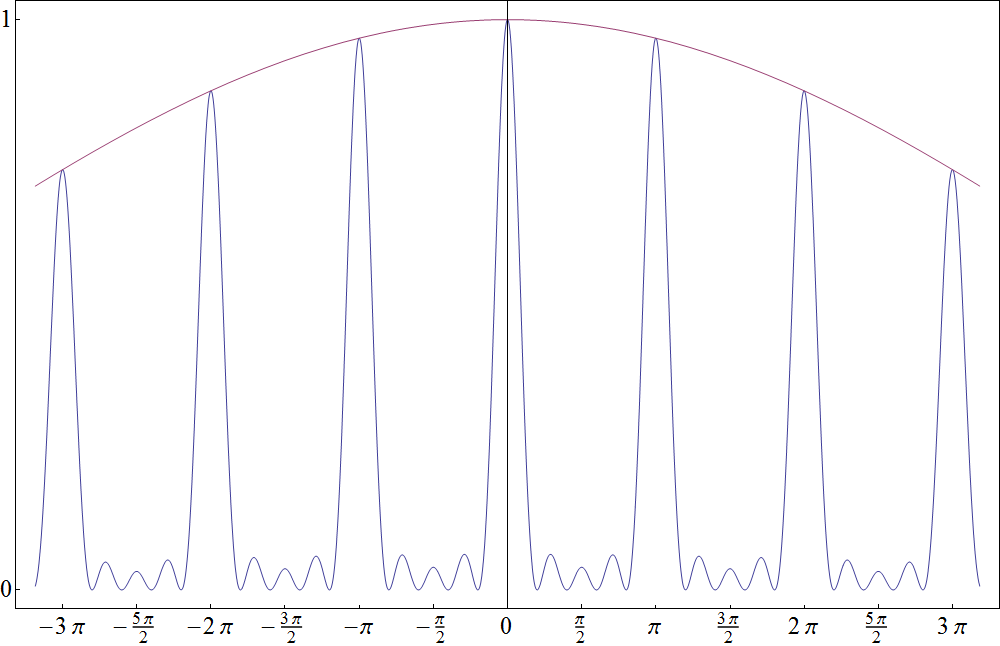
\includegraphics[width=\textwidth]{difraccion_rendijas_a_chico}
                \caption{a = 0.01b}
                \label{fig:difraccion_red_rendija_a_chico}
        \end{subfigure}
        \qquad
        \begin{subfigure}[b]{0.3\textwidth}
                \centering
                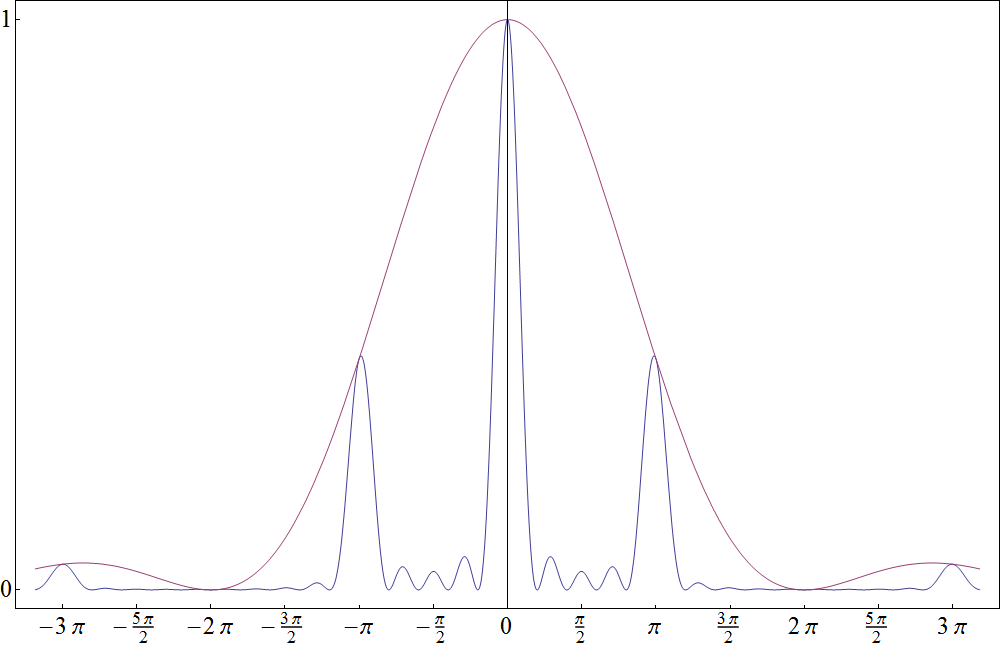
\includegraphics[width=\textwidth]{difraccion_rendijas_a_grande}
                \caption{a = 0.1b}
                \label{fig:difraccion_red_rendija_a_grande}
        \end{subfigure}
        \caption{Patrones para 5 aberturas con diferentes tamañaos}\label{fig:difraccion_red_rendijas_irradiancia}
\end{figure}
	
	Para resolver aberturas bidimensionales consideremos un diferencial de campo producto de un diferencial de superficie \[ dE = \frac{\varepsilon}{R} e^{i (k r - \omega t)} dS.\] En este caso la distancia $r$ seguirá $r^2 = X^2 + (Y - y)^2 + (Z - z)^2$, donde las coordenadas en mayúscula representan el punto $P$ y las minusculas las coordenadas del plano de la abertura; de esta forma $r^2 = R^2 + (x^2 +z^2) - 2(Yy - Zz)$ y si hacemos un desarrollo de Taylor a primer orden obtenemos que \[r = R \left(1 - \frac{Yy - Zz}{R^2}\right)\] por lo que la integral nos queda
	\begin{equation}
		E = \frac{\varepsilon}{R} e^{i(\omega t - k R)} \int_{\text{abertura}} e^{i k \frac{Yy - Zz}{R}} dS
		\label{eq:difraccion_abertura_bidimensional}
	\end{equation}
	que podemos escribir de la siguiente manera, consolidando las constantes en la función $A(x,y)$ y observamos que $k_Y = k \frac{Y}{R}$ y lo mismo para $k_Z$
	\begin{equation}
		E(x,y) = \iint A(x',y') e^{i (k_Y y + k_Z z)} dx dy
		\label{eq:difraccion_general}
	\end{equation}
	donde queda evidente que el campo finalmente va a ser la transformada de Fourier de la función $A$ que llamamos función de abertura.
	
	Haciendo la integral \ref{eq:difrracion_abertura_bidimensional} para una ranura rectangular, con lado $a$ en el eje $z$ y lado b en el eje $y$, encontramos que tiene una irrandiancia compuesta por dos irradiancias en el eje $y$ y en el eje $z$ (ya que la integral se puede separar en virtud del teorema de Fubini), es decir
	\begin{equation}
		I(\beta_y = k b Y / 2 R, \beta_y = k a Z / 2 R) = I(0) \text{senc}^2(\beta_y) \text{senc}^2(\beta_z)
	\end{equation}
	Para una abertura circular, radio $a$, debemos escribir la integral en coordenadas esféricas y utilizar la función $J_0$ de Bessel, que es igual a \[J_0(u) = \frac{1}{2\pi} \int_0^{2\pi} e^{i u \cos(v)} dv,\] la cual al integrarla nos queda un campo igual a \[ E = \frac{\varepsilon e^{i(\omega t - k R)}}{k q} 2 \pi a J_1\left(\frac{k a q}{R}\right)\] donde $q$ es la distancia en el plano imagen al punto $P$. De esta forma la irradiancia queda 
	\begin{equation}
		I(\theta) = 4 I_0 \frac{J_1^2(k a \sen(\theta))}{k a \sen(\theta)}
		\label{eq:difraccion_circular_irradiancia}
	\end{equation}
	Acá podemos observar que el máximo central tiene una extensión radial, que numéricamente observamos igual a 
	\begin{equation}
		q_1 = 1,22\frac{R\lambda}{2 a}
	\end{equation}
	valor que va a determinar, por ejemplo, el límite de una lente que enfoca en la pantalla (es decir $f \approx R$) debido a la difracción. 
	La expresión anterior  determina el criterio de Rayleigh para resolver imagenes; en este criterio es necesario que el máximo central del patrón de cada imagen esté el en minimo de la otra, así es posible diferenciar las dos fuentes.
	\subsection{Redes de difracción}
		Una red de difracción corresponde a un objeto con un patrón periodico que difracta de forma periodica la luz entrante, por medio de cambio periodo de fase u/o amplitud. Para las redes de amplitud, utilizamos la irradiancia de la ecuación \ref{eq:difraccion_red_rendijas_irradiancia}, ya que una colección de $N$ rendijas es básicamente una red de difracción por amplitud (sea por reflexión o transmisión). De esa forma nos queda que
		\begin{equation}
			a (\sen(\theta_m) - \sen(\theta_i)) = m \lambda
			\label{eq:difraccion_red_ecuacion}
		\end{equation}
		que es de caracter general, aún para las redes por cambio de fase (donde podemos encontrar la diferencia de camino óptico por medio de un esquema), donde $\theta_i$ es el ángulo de incidencia respecto a la normal de la red.
		
		Finalmente definimos la resolución espectral de una red como la capacidad de generar máximos para longitudes de onda cercanas, es decir
		\begin{equation}
			R = \frac{\lambda}{\Delta \lambda_{\text{min}}}
			\label{eq:difraccion_red_resolucion_espectral}
		\end{equation}
		y si consideramos el criterio de Rayleigh (que el máximo central de una longitud de onda esté en el primer minimo de la más cercana) obtenemos que \[R = m N,\] que finalmente nos queda
		\begin{equation}
			R = \frac{N a(\sen(\theta_m) - \sen(\theta_i)}{\lambda}
			\label{eq:difraccion_red_resolucion_rayleigh}
		\end{equation}
		donde podemos deducir que en autocolimación ($\theta_i = -\theta_m = 90^\circ$) logramos la mayor resolución espectral.
\begin{thebibliography}{9}
    \bibitem{martinez}
        Oscar E. Martinez, \emph{Ondas: es física}
	\bibitem{pain}
		H. J. Pain, \emph{The physics of vibrations and waves}
    \bibitem{crawford}
        Frank J. Crawford, \emph{Ondas}

	\bibitem{hetch}
		E. Hetch, \emph{Óptica}
\end{thebibliography}
%\newpage
%\appendix
%\section{Transformada de Fourier}
\end{document}
